\section{Implementation on a disk}
First we recall that the organization of files as sets of individually allocated blocks (sectors) is
inherently required by the allocation considerations of dynamically growing sequences. However,
if the storage medium is a tape, a disk, or a flash-RAM, there exists an additional reason for the
use of blocks. They constitute the subsequences to be individually buffered for transmission in
order to overcome the timing constraints imposed by the medium. If an adequate space utilization
is to be achieved, the blocks must not be too long. A typical size is 1, 2, or 4K bytes.
This necessity of buffering has a profound influence on the implementation of file access. The
complication arises because the abstraction of the sequence of individual bytes needs to be
maintained. The increase in complexity of file access is considerable, as can be seen by
comparing the program listings of the 2 respective implementations.

The first, obvious measure is to copy the file's sector table into primary store when a file is
"opened" through a call of \verb|New()| or \verb|Old()|. The record holding this copy is the file
descriptor, and the value \verb|f| denoting the file points to this handle (instead of the actual header
on disk). The descriptor also contains the remaining information stored in the header, in particular
the file's length.

If a file is read (or written) in purely sequential manner, a single buffer is appropriate for the
transfer of data. For reading, the buffer is filled by reading a sector from the disk, and bytes are
picked up individually from the buffer. For writing, bytes are deposited individually, and the buffer
is written onto disk as a whole when full. The buffer is associated with the file, and a pointer to it
is contained in the descriptor.

However, we recall that several riders may be placed on a file and be moved independently. It might be
appealing to associate a buffer with each rider. But this proposal must quickly be rejected when we
realize that several riders may be active at neighbouring positions. If these positions refer to the
same sector, which is duplicated in the riders' distinct buffers, the buffers may easily become
inconsistent. Obviously, buffers must not be associated with riders, but with the file itself. The
descriptor therefore contains the head of a list of linked buffers. Each buffer is identified by its
position in the file. An invariant of the system is that no 2 buffers represent the same sector.

Even with the presence of a single rider, the possibility of having several buffers associated with a
file can be advantageous, if a rider is frequently repositioned. It becomes a question of strategy and
heuristics when to allocate a new buffer. In the Oberon, we have adopted the following solution:
\begin{enumerate}
  \item The first buffer is created when the file is opened (\verb|New|, \verb|Old|).
  \item Additional buffers may be allocated when a rider is placed (or repositioned) on the file.
  \item At most four buffers are connected to the same file.
  \item Purely sequential movements of riders do not cause allocation of buffers.
  \item Separate buffers are generated when extensions of the file's sector table need be accessed
    (rider position > 64K). Each buffers the 256 sector addresses of the respective index sector.
\end{enumerate}

The outlined scheme requires and is based upon the following data structures and types:
\begin{verbatim}
  File   = POINTER TO FileDesc;
  Buffer = POINTER TO BufferRecord;
  Index  = POINTER TO IndexRecord;

FileDesc = RECORD next: File;
             aleng, bleng: INT;      (*file length*)
             nofbufs: INT;           (*no. of buffers allocated*)
             modH, registered: BOOL; (*header has been modified*)
             firstbuf: Buffer:       (*head of buffer chain*)
             sechint: DiskAdr;       (*sector hint*)
             name: FileDir.FileName;
             date: INT;
             ext: ARRAY FileDir.ExTabSize OF Index;
             sec: ARRAY 64 OF DiskAdr
           END;

BufferRecord = RECORD apos, lim: INT; (*lim = no. of bytes*)
                 mod: BOOL;    (*buffer has been modified*)
                 next: Buffer; (*buffer chain*)
                 data: FileDir.DataSector
               END;

IndexRecord = RECORD adr: DiskAdr;
                mod: BOOL; (*index record has been modified*)
                sec: FileDir.IndexSector
              END;

Rider = RECORD eof: BOOL;   (*end of file reached*)
          res: INT;         (*no. of unread bytes*)
          file: File;
          apos, bpos: INT;  (*position*)
          buf: Buffer       (*hint: likely buffer*)
        END ;
\end{verbatim}

In order to increase efficiency of access, riders have been provided with a field containing the address
of the element of the rider's position. From the conditions stated above for the allocation of buffers,
it is evident that the value of this field can be a hint only. This implies that there can be no
reliance on its information. Whenever it is used, its validity has to be checked. The check consists in
a comparison of the riders' position \verb|r.apos| with the hinted buffer's actual position
\verb|r.buf.apos|. If they differ, a buffer with the desired position must be searched and, if not
present, allocated. The advantage of the hint lies in the fact that the hint is correct with a very high
probability. The check is included in procedures \verb|Read|, \verb|ReadByte|, \verb|Write|, and
\verb|WriteByte|.

Some fields of the record types require additional explanations:
\begin{enumerate}
  \item The length is stored in a "preprocessed" form, namely by the 2 integers \verb|aleng| and
    \verb|bleng| such that \verb|aleng| is a sector number and
    \begin{verbatim}
      length = (aleng * SS) + bleng - HS
      aleng = (length + HS) DIV SS
      bleng = (length + HS) MOD SS
    \end{verbatim}
    The same holds for the form of the position in riders (\verb|apos|, \verb|bpos|).
  \item The field \verb|nofbufs| indicates the number of buffers in the list headed by \verb|firstbuf|:
    \begin{verbatim}
      1 <= nofbufs <= Maxbufs.
    \end{verbatim}
  \item Whenever data are written into a buffer, the file becomes inconsistent, i.e. the data on the
    disk are outdated. The file is updated, i.e. the buffer is copied into the corresponding disk
    sector, whenever the buffer is reallocated, e.g. during sequential writing after the buffer is full
    and is "advanced". During sequential reading, a buffer is also advanced and reused, but needs not be
    copied onto disk, because it is still consistent. Whether a buffer is consistent or not is indicated
    by its state variable \verb|mod| (modified). Similarly, the field \verb|modH| in the file descriptor
    indicates whether or not the header had been modified.
  \item The field \verb|sechint| records the number of the last sector allocated to the file and serves
    as a hint to the kernel's allocation procedure, which allocates a next sector with an address larger
    than the hint. This is a measure to gain speed in sequential scans.
  \item The buffer's position is specified by its field \verb|apos|. Used as index in the file header's
    sector table, it yields the sector corresponding to the current buffer contents. The field
    \verb|lim| specifies the number of bytes \verb|s| stored in the buffer. Reading cannot proceed
    beyond this limiting index; writing beyond it implies an increase in the file's length. All buffers
    except the one for the last sector are filled and specify \verb|lim = SS|.
  \item The hidden rider field \verb|buf| is merely a hint to speed up localization of the concerned
    buffer. A hint is likely, but not guaranteed to be correct. Its validity must be checked before use.
    The buffer hint is invalidated when a buffer is reallocated and/or a rider is repositioned.  The
    structure of riders remains practically the same as for files using main store. The hidden field
    \verb|adr| is merely replaced by a pointer to the buffer covering the rider's position. A
    configuration of a file \verb|f| with 2 riders is shown in Fig \ref{fig:file}.
    \begin{figure}
      \flushright
      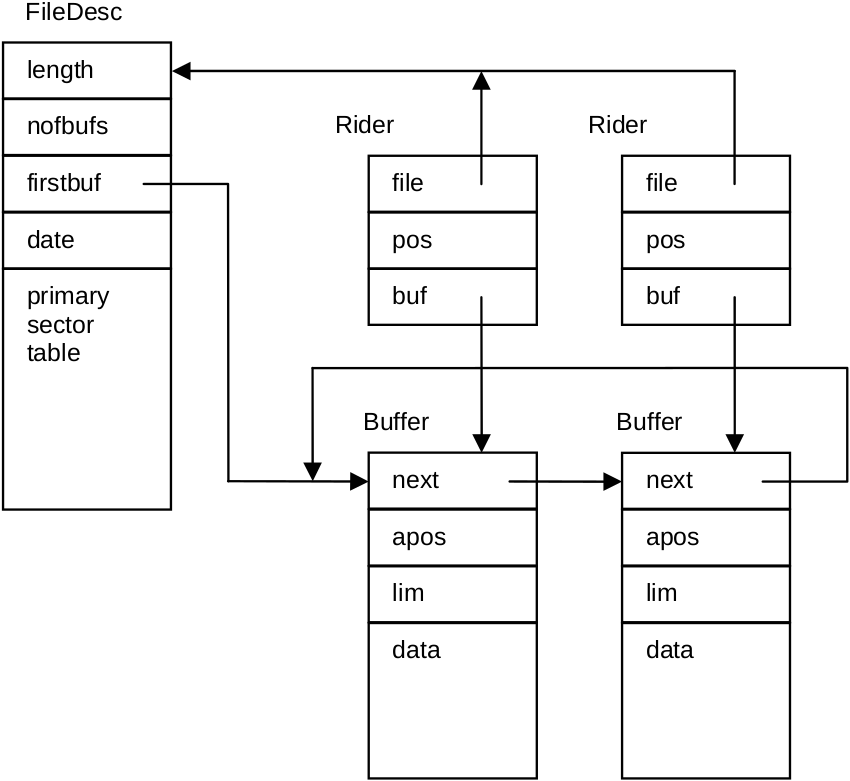
\includegraphics[width=.9\textwidth]{i/m}
      \caption{File $f$ with 2 riders and 2 buffers}
      \label{fig:file}
    \end{figure}
\end{enumerate}

Some comments concerning module \verb|Files| follow.
\begin{enumerate}
  \item After the writing of a file has been completed, its name is usually registered in the directory.
    Register invokes procedure \verb|Unbuffer|. It inspects the associated buffers and copies those onto
    disk which had been modified. During this process, new index sectors may have to be transferred
    as well. If a file is to remain anonymous and local to a module or command, i.e. is not to be
    registered, but merely to be read, the release of buffers must be specified by an explicit call to
    \verb|Close| (meaning "close buffers"), which also invokes \verb|Unbuffer|.
  \item Procedure \verb|Old| (and for reasons of consistency also \verb|New|) deviates from the general
    Oberon programming rule that an object be allocated by the calling (instead of the called) module.
    This rule would suggest the statements \verb|New(f); Files.Open(f, name)| instead of
    \verb|f := Files.Old(name)|. The justification for the rule is that any extension of the type of
    \verb|f| could be allocated, providing for more flexibility. And the reason for our deviation in the
    case of files is that, upon closer inspection, not a new file, but only a new descriptor is to be
    allocated.  The distinction becomes evident when we consider that several statements
    \verb|f := Files.Old(name)| with different \verb|f| and identical name may occur, probably in
    different modules. In this case, it is necessary that the same descriptor is referenced by the
    delivered pointers in order to avoid file inconsistency. Each (opened) file must have exactly one
    descriptor. When a file is opened, the first action is therefore to inspect whether a descriptor of
    this file already exists. For this purpose, all descriptors are linked together in a list anchored
    by the global variable \verb|root| and linked by the descriptor field \verb|next|. This measure may
    seem to solve the problem of avoiding inconsistencies smoothly. However, there exists a pitfall that
    is easily overlooked: All opened files would permanently remain accessible via \verb|root|, and the
    garbage collector could never remove a file descriptor nor its associated buffers. This would be
    unacceptable. In order to hide this list from the garbage collector, it is represented by integers
    (addresses) instead of pointers.
  \item Sector pointers are represented by sector numbers of type \verb|INT|. Actually, we use the
    numbers multiplied by 29. This implies that any single-bit error leads to a number which is not a
    multiple of 29, and hence can easily be detected. Thereby the crucial sector addresses are
    software parity checked and are safe (against single-bit errors) even on computers without hardware
    parity check. The check is performed by procedures \verb|Kernel.GetSector| and
    \verb|Kernel.PutSector|.
\end{enumerate}
